% Provenance (never printed): old terminale S material on the transformation of
% rocks in mountain belts and subduction zones (pressure, temperature, index
% minerals and the Al2SiO5 polymorphs, foliation, contact and regional
% metamorphism). Owner (Sync 0): metamorphism, lithostatic pressure, polymorph,
% index mineral/isograd/metamorphic grade, foliation/schistosity, contact and
% regional metamorphism/aureole. Blueschist and eclogite are g11.06's, the
% geotherm g11.03's, minerals and silicates g11.07's, the rock families, marble
% and slate Book 1's (g6), pressure physics': recalled, never redefined. The
% P-T diagram: figdata/grade-12/al2sio5.py (Holdaway and Mukhopadhyay 1993,
% Table 11; geotherms from Earle 7.3).
\chapter{As rochas metamórficas}\label{ch:g12:metamorphic-rocks}

Uma camada de lama se deposita num fundo de mar e endurece em folhelho.
Enterre-a alguns quilômetros e comprima-a, e ela vira uma ardósia, uma rocha
que se parte nas placas finas e planas de um telhado. Enterre-a mais fundo e
mais quente, e as suas pequenas escamas crescem em micas brilhantes, entre
as quais incham granadas vermelhas: um xisto. Mais fundo e mais quente
ainda, os seus minerais se separam em faixas claras e escuras: um gnaisse.
Nada se fundiu no caminho. A mesma lama, com os mesmos elementos químicos,
simplesmente reconstruiu os seus minerais para se adaptar ao lugar onde
estava. Lidos no sentido inverso, os minerais de uma rocha metamórfica
registram quão fundo e quão quente era esse lugar, e este capítulo aprende a
lê-los.
% ledger: earle:foliation, earle:settings

\begin{recall}
As rochas se dividem em três famílias --- ígneas, sedimentares,
metamórficas ---, e o ciclo das rochas transforma umas nas outras; o mármore
se forma a partir do calcário e a ardósia a partir do folhelho, sem fusão
(Livro 1, 6º ano). Um mineral é um sólido natural de composição química
definida e com um arranjo ordenado de átomos; a maioria dos minerais da
crosta são \omterm{def:g11:minerals:silicate}{silicatos} (\cref{ch:g11:minerals}). Uma \omterm{def:g11:lithosphere-asthenosphere:geotherm}{geoterma} é a curva da
temperatura em função da profundidade sob um lugar; perto da superfície, a
temperatura sobe de 25 a \qty{30}{\celsius} por quilômetro
(\cref{ch:g11:lithosphere-asthenosphere}). Numa \omterm{def:g11:subduction-zones:subduction}{zona de subducção}, a \omterm{def:g11:ocean-ridges:oceanic-lithosphere}{crosta
oceânica} levada para baixo enquanto continua fria se transforma em \omterm{def:g11:subduction-zones:eclogite}{xisto
azul}, depois em \omterm{def:g11:subduction-zones:eclogite}{eclogito} (\cref{ch:g11:subduction-zones}). A pressão é uma
força dividida pela área sobre a qual ela age; ela se mede em pascals,
\qty{1}{Pa} = \qty{1}{N/m^2}.
\end{recall}
% ledger: usgs:metamorphic (Book 1 row), webmineral:formulas, earle:settings, earle:controls

\section{Transformadas no estado sólido}

\begin{definition}[Metamorfismo]\label{def:g12:metamorphic-rocks:metamorphism}
O \emph{metamorfismo}\index{metamorfismo} é a transformação dos minerais e da
\omterm{def:g11:igneous-rocks:texture}{textura} de uma rocha, no estado sólido, quando ela é levada a uma
temperatura e a uma pressão diferentes daquelas sob as quais se formou. A
rocha em que ela se transforma é uma rocha metamórfica.
\end{definition}
% ledger: tulane:metamorphism, earle:controls

A rocha de onde o \omterm{def:g12:metamorphic-rocks:metamorphism}{metamorfismo} parte é a sua \omterm{def:g10:soil-formation:weathering-profile}{rocha-mãe}, a mesma palavra que
para a rocha sob um solo (\cref{ch:g10:soil-formation}). O \omterm{def:g12:metamorphic-rocks:metamorphism}{metamorfismo}
começa a cerca de \qty{200}{\celsius}; abaixo disso, as lentas mudanças de
um sedimento enterrado fazem parte do seu endurecimento em rocha. Ele
termina onde a rocha começa a se fundir: a partir daí, o que acontece é
ígneo. Entre esses limites, cada mineral só é estável numa certa faixa de
temperatura e de pressão. A maioria dos \omterm{def:g10:soil-formation:clay}{argilominerais}, por exemplo, só
dura até cerca de 150 ou \qty{200}{\celsius}; acima disso, eles se
transformam em micas. Quando as condições mudam, os átomos dos minerais
instáveis se rearranjam, grão por grão, em minerais estáveis nas novas
condições.
% ledger: tulane:metamorphism, earle:controls

Quatro fatores controlam o resultado. A \textbf{\omterm{def:g10:soil-formation:weathering-profile}{rocha-mãe}} fornece os
elementos químicos: um calcário feito só de calcita só pode virar um
mármore feito de calcita. A \textbf{temperatura} e a \textbf{pressão} decidem quais
minerais são estáveis. E a \textbf{água}, presente em pequenas quantidades
entre os grãos, leva íons dissolvidos de um grão ao seguinte e acelera as
reações. O \omterm{def:g12:metamorphic-rocks:metamorphism}{metamorfismo} é lento: os novos minerais crescem cerca de um
milímetro em um milhão de anos. Os eventos tectônicos que enterram as
rochas também são lentos, por isso as reações costumam ter tempo de se
completar.
% ledger: earle:controls

\subsection{O peso das rochas de cima}

Uma rocha enterrada a uma profundidade $z$ suporta o peso de toda a rocha
acima dela.

\begin{definition}[Pressão litostática]\label{def:g12:metamorphic-rocks:lithostatic}
A \emph{pressão litostática}\index{pressao litostatica@pressão litostática} a uma profundidade $z$
é a pressão exercida sobre uma rocha pelo peso da coluna de rocha acima
dela. Ela é a mesma em todas as direções.
\end{definition}
% ledger: earle:controls (confining pressure, equal in all directions), tulane:metamorphism

\begin{proposition}[Pressão litostática]\label{prop:g12:metamorphic-rocks:lithostatic}
Sob uma coluna de rocha de densidade uniforme $\rho$, a \omterm{def:g12:metamorphic-rocks:lithostatic}{pressão litostática}
à profundidade $z$ é
\[
  P = \rho g z ,
\]
em que $g$ é a aceleração da gravidade; a pressão da atmosfera, cerca de
\qty{0.1}{MPa}, é desprezada.
\end{proposition}

\begin{proof}
Tome uma coluna vertical de rocha de seção horizontal $A$, da superfície
até a profundidade $z$. O seu volume é $Az$, a sua massa $\rho A z$, e o seu
peso $\rho A z g$. Esse peso repousa sobre a área $A$ da base da coluna,
logo a pressão ali é $P = \rho A z g / A = \rho g z$.
\end{proof}

Com a densidade média da \omterm{def:g12:continental-crust:continental-crust}{crosta continental}, $\rho = \qty{2830}{kg/m^3}$, e
$g = \qty{9.81}{m/s^2}$, a pressão sobe de $\rho g = 2830 \times 9.81
\approx \qty{27800}{Pa}$ por metro, isto é, cerca de \qty{27.8}{MPa} por
quilômetro. Na base de uma crosta de \qty{35}{km} de espessura, ela atinge
\[
  P = 2830 \times 9.81 \times \num{35000} \approx \qty{9.7e8}{Pa} \approx
  \qty{0.97}{GPa},
\]
cerca de \qty{1}{GPa}: quase dez mil vezes a pressão da atmosfera ao nível
do mar. As pressões são muitas vezes lidas ao contrário, como
profundidades: \qty{1}{GPa} é atingido a
$\num{e9}/(2830 \times 9.81) \approx \qty{36}{km}$ de profundidade.
% values: P_35km_gpa 0.97168, dPdz_mpa_per_km 27.762, z_1gpa_km 36.02 (al2sio5.py)
% ledger: cm95:crust; Book 1: ussa76:sea-level (101 325 Pa, g0 = 9.80665 m/s2)

O peso das rochas pressiona igualmente de todos os lados. Num cinturão de
montanhas, as placas acrescentam um empurrão numa direção: a rocha é
comprimida com mais força pelos lados do que por cima. Essa pressão
\emph{dirigida} não muda quais minerais são estáveis, mas muda a maneira
como eles se arranjam, como mostra a \cref{sec:g12:metamorphic-rocks:foliation}.
% ledger: earle:controls (directed pressure), earle:foliation

\section{Minerais índice e grau}

\subsection{Três minerais de uma só fórmula}

\begin{definition}[Polimorfo]\label{def:g12:metamorphic-rocks:polymorph}
Dois minerais são \emph{polimorfos}\index{polimorfo} quando têm a mesma
composição química mas estruturas cristalinas diferentes: os mesmos átomos,
arranjados de outro modo.
\end{definition}
% ledger: earle:controls

Três minerais compartilham a fórmula \ce{Al2SiO5}: a cianita, a andaluzita e
a silimanita. Cada um é estável na sua própria faixa de temperatura e de
pressão, medida em laboratório mantendo cristais a uma temperatura e a uma
pressão escolhidas e observando qual \omterm{def:g12:metamorphic-rocks:polymorph}{polimorfo} cresce às custas do outro. A
cianita é o mais denso dos três,
\qty{3.61}{g/cm^3} contra \qty{3.24}{g/cm^3} para a silimanita e
\qty{3.15}{g/cm^3} para a andaluzita: os seus átomos estão mais compactados,
e é ela que as altas pressões favorecem.
% ledger: earle:controls, hm93:triple, hm93:table11; Book 3: webmineral:polymorphs (densities)

\begin{omfigure}
\begin{tikzpicture}
\begin{axis}[omrecord, name=pt, scale only axis, width=0.62\linewidth, height=6.4cm,
  xmin=200, xmax=900, ymin=0, ymax=1.2, y dir=reverse,
  xlabel={temperatura (\unit{\celsius})}, ylabel={pressão (\unit{GPa})},
  xtick={200,300,...,900}, ytick={0,0.2,...,1.2},
  yticklabel style={/pgf/number format/fixed, /pgf/number format/precision=1},
  axis y line*=left]
% computed in figdata/grade-12/al2sio5.py from Holdaway and Mukhopadhyay (1993), Table 11
\addplot[omDef, line width=0.9pt, densely dashed] table[x=T10, y=P_GPa] {figdata/out/grade-12-al2sio5-geotherms.dat};
\addplot[omMeth, line width=0.9pt, densely dashed] table[x=T30, y=P_GPa] {figdata/out/grade-12-al2sio5-geotherms.dat};
\addplot[omThm, line width=0.9pt, densely dashed] table[x=T50, y=P_GPa] {figdata/out/grade-12-al2sio5-geotherms.dat};
\addplot[black, line width=1.2pt] table[x=T, y=P_GPa] {figdata/out/grade-12-al2sio5-andky.dat};
\addplot[black, line width=1.2pt] table[x=T, y=P_GPa] {figdata/out/grade-12-al2sio5-kysil.dat};
\addplot[black, line width=1.2pt] table[x=T, y=P_GPa] {figdata/out/grade-12-al2sio5-andsil.dat};
\addplot[black, line width=1.2pt, dotted] table[x=T, y=P_GPa] {figdata/out/grade-12-al2sio5-andsilx.dat};
\addplot[only marks, mark=*, mark size=2pt, black] coordinates {(504.2,0.3758)};
\addplot[only marks, mark=o, mark size=2pt, line width=0.8pt, black] coordinates {(573.6,0.5216) (340.1,0.1833) (553.0,0.3015)};
\coordinate (ky) at (axis cs:370,0.55);
\coordinate (and) at (axis cs:470,0.12);
\coordinate (sil) at (axis cs:765,0.57);
\coordinate (tp) at (axis cs:504.2,0.3758);
\coordinate (g10) at (axis cs:415,1.0);
\coordinate (g30) at (axis cs:206,0.36);
\coordinate (g50) at (axis cs:895,0.355);
\end{axis}
\begin{axis}[scale only axis, width=0.62\linewidth, height=6.4cm, at={(pt.south west)}, anchor=south west,
  xmin=200, xmax=900, ymin=0, ymax=43.224, y dir=reverse, axis x line=none, axis y line*=right,
  axis line style={-}, ylabel={profundidade (\unit{km})}, ytick={0,5,...,40},
  every axis label/.append style={font=\small}, tick label style={font=\small}]
\end{axis}
\node[font=\small\bfseries] at (ky) {cianita};
\node[font=\small\bfseries] at (and) {andaluzita};
\node[font=\small\bfseries] at (sil) {silimanita};
\node[font=\scriptsize, text=omDef, anchor=west, inner sep=1pt] at (g10) {\qty{10}{\celsius/km}, zona de subducção};
\node[font=\scriptsize, text=omMeth!70!black, anchor=north west, inner sep=1pt, align=left] at (g30) {\qty{30}{\celsius/km},\\típica};
\node[font=\scriptsize, text=omThm, anchor=south east, inner sep=1pt] at (g50) {\qty{50}{\celsius/km}, região vulcânica};
\end{tikzpicture}

{\small Os campos dos três \omterm{def:g12:metamorphic-rocks:polymorph}{polimorfos} de \ce{Al2SiO5}, com a pressão
crescendo para baixo como a profundidade (escala da direita, para uma crosta
de densidade \qty{2830}{kg/m^3}). Linhas pretas: os limites medidos em
laboratório; os três se encontram no ponto triplo (ponto preto),
\qty{504}{\celsius} e \qty{0.375}{GPa}. Tracejadas: três \omterm{def:g11:lithosphere-asthenosphere:geotherm}{geotermas}, que
partem de \qty{10}{\celsius} na superfície; os círculos marcam onde elas
cruzam um limite.}
\end{omfigure}
% values: triple_T 504.21, triple_P_gpa 0.37584, triple_z_km 13.538; crossings 30: 573.6 degC 18.79 km; 50: 340.1 degC 6.60 km, 553.0 degC 10.86 km (al2sio5.py)
% ledger: hm93:table11, hm93:triple, cm95:crust, earle:settings

O diagrama é um mapa de estabilidade. Cada ponto é uma temperatura e uma
pressão; cada campo é o \omterm{def:g12:metamorphic-rocks:polymorph}{polimorfo} estável ali. A cianita ocupa as altas
pressões, a andaluzita as baixas pressões e as temperaturas moderadas, a
silimanita as altas temperaturas. Ao longo de um limite, dois \omterm{def:g12:metamorphic-rocks:polymorph}{polimorfos} são
igualmente estáveis, e no ponto triplo, os três. Os limites não são
conhecidos com exatidão: o ponto triplo tem uma incerteza de cerca de
\qty{20}{\celsius} e \qty{0.025}{GPa}, e traços de ferro nos cristais
deslocam a linha andaluzita--silimanita em até \qty{20}{\celsius}.
% ledger: hm93:triple

\begin{method}[Ler um diagrama pressão--temperatura]\label{met:g12:metamorphic-rocks:pt}
\begin{enumerate}
  \item Situe o ponto da rocha: a sua temperatura no eixo horizontal, a sua
        pressão no vertical.
  \item Leia o campo em que ele cai: o mineral estável ali.
  \item Converta a pressão numa profundidade com $z = P/(\rho g)$, ou leia-a
        na escala de profundidade.
  \item Para um mineral encontrado numa rocha, leia no sentido inverso: a
        rocha estava no campo desse mineral quando ele se cristalizou. Dois
        minerais que se formaram juntos, ou um mineral que falta, estreitam
        ainda mais a faixa.
\end{enumerate}
\end{method}

\begin{example}[O limite cianita--silimanita]\label{ex:g12:metamorphic-rocks:kysil}
A \qty{0.6}{GPa}, a cianita se transforma em silimanita a cerca de
\qty{611}{\celsius}. Essa pressão é atingida a $z = \num{0.6e9} / (2830
\times 9.81) \approx \qty{21.6}{km}$. Entre 600 e \qty{700}{\celsius}, o
limite sobe \qty{0.209}{GPa}, isto é, $0.209/0.0278 \approx
\qty{7.5}{km}$ de profundidade: uma rocha \qty{7.5}{km} mais funda precisa
estar cerca de \qty{100}{\celsius} mais quente para se transformar em
silimanita. Um xisto que contém cianita mas nenhuma silimanita e que se
cristalizou a \qty{21.6}{km} estava, portanto, mais frio que cerca de
\qty{611}{\celsius}.
\end{example}
% values: kysil_T_at_6kbar 611, kysil_z_at_6kbar 21.612, kysil_slope 2.09 kbar per 100 degC, dPdz 27.762 MPa/km (al2sio5.py)

\subsection{Minerais índice e isógradas}

Num cinturão de rochas que começaram todas como a mesma lama, os minerais
mudam de um lugar para outro, porque as rochas não foram todas enterradas
tão fundo nem aquecidas tanto.

\begin{definition}[Mineral índice; isógrada; grau metamórfico]\label{def:g12:metamorphic-rocks:index-mineral}
O \emph{grau metamórfico}\index{grau metamorfico@grau metamórfico} de uma rocha é a
intensidade do \omterm{def:g12:metamorphic-rocks:metamorphism}{metamorfismo} que ela sofreu, fixada pela temperatura e pela
pressão que ela atingiu. Um \emph{mineral índice}\index{mineral indice@mineral índice} é um
mineral cujo primeiro aparecimento, em rochas de mesma composição de
origem, marca um dado grau. Uma \emph{isógrada}\index{isograda@isógrada} é a linha num mapa
(uma superfície no terreno) que une os lugares onde um mineral índice
aparece pela primeira vez: ao longo dela, as rochas atingiram o mesmo grau.
\end{definition}
% ledger: tulane:metamorphism, earle:regional

As rochas formadas a partir de lama, ricas em alumínio, mostram a sequência
mais clara. Com o aumento do grau, os \omterm{def:g12:metamorphic-rocks:index-mineral}{minerais índice} aparecem na ordem
clorita, biotita, granada, estaurolita, cianita, silimanita, e o terreno
que eles dividem se chama zona da clorita, zona da biotita, e assim por
diante. A temperatura e a pressão sobem ambas ao longo dessa sequência, como
numa crosta espessada sob um cinturão de montanhas.
% ledger: iugs:barrow, earle:regional

\begin{omfigure}
\begin{tikzpicture}[font=\scriptsize]
  \def\zone#1#2#3#4{\fill[#1] (#2,0) ellipse ({#3} and {#4});}
  \zone{omProp!8}{0}{6.6}{2.55}
  \zone{omProp!18}{0.5}{5.4}{2.2}
  \zone{omProp!32}{1.0}{4.3}{1.82}
  \zone{omThm!28}{1.4}{3.2}{1.44}
  \zone{omThm!45}{1.8}{2.1}{1.06}
  \zone{omThm!65}{2.2}{1.0}{0.66}
  \foreach \c/\a/\b in {0.5/5.4/2.2, 1.0/4.3/1.82, 1.4/3.2/1.44, 1.8/2.1/1.06, 2.2/1.0/0.66}
    \draw[black!70, line width=0.6pt] (\c,0) ellipse ({\a} and {\b});
  \draw[black!40] (0,0) ellipse (6.6 and 2.55);
  \node at (-5.75,0) {clorita};
  \node at (-4.1,0) {biotita};
  \node at (-2.55,0) {granada};
  \node at (-1.05,0) {estaurolita};
  \node at (0.45,0) {cianita};
  \node[text=white, font=\scriptsize\bfseries] at (2.2,0) {silimanita};
  \draw[omDef, -{Stealth}, line width=0.8pt] (5.6,-2.6) node[right, text=omDef] {o grau sobe} -- (3.0,-0.65);
  \draw[black!70] (3.76,1.394) -- (5.8,2.2) node[right, align=left] {isógrada\\da granada};
\end{tikzpicture}

{\small Um mapa esquemático de zonas metamórficas em rochas formadas a
partir de lama: cada \omterm{def:g12:metamorphic-rocks:index-mineral}{isógrada} (linha preta) marca o primeiro aparecimento de
um \omterm{def:g12:metamorphic-rocks:index-mineral}{mineral índice}, e o grau sobe em direção ao núcleo do cinturão, onde as
rochas foram enterradas mais fundo e aquecidas mais. As zonas reais são
curvadas e cortadas por \omterm{def:g12:mountain-building:fold}{dobras} e falhas; as suas larguras aqui são
arbitrárias.}
\end{omfigure}
% ledger: iugs:barrow, earle:regional

\begin{history}[As zonas de Barrow]
Na década de 1890, o geólogo George Barrow mapeou os xistos e os gnaisses
das Terras Altas da Escócia e notou que os seus minerais mudavam através da
região numa ordem regular. Ele foi o primeiro a dividir uma região em zonas
pelos minerais que as suas rochas contêm. O seu nome ficou para a
sequência: diz-se que as rochas que a seguem mostram um \omterm{def:g12:metamorphic-rocks:metamorphism}{metamorfismo}
\emph{barroviano}.
\end{history}
% ledger: earle:regional, barrow1893:paper, iugs:barrow

O grau também pode ser estimado grosseiramente só pela temperatura. As
rochas aquecidas de 150 a \qty{300}{\celsius} são de grau muito baixo, de
300 a \qty{450}{\celsius} de grau baixo, de 450 a \qty{550}{\celsius} de
grau médio, e acima de \qty{550}{\celsius} de grau alto. No grau baixo, as
rochas são ricas em minerais que contêm água na sua estrutura, como as
argilas e a clorita; à medida que o grau sobe, elas perdem essa água.
% ledger: earle:foliation (Table 7.1 grades), tulane:metamorphism

\section{A foliação}\label{sec:g12:metamorphic-rocks:foliation}

Comprimidos enquanto crescem, os minerais não crescem em todas as direções.
Os grãos achatados, como as micas, e os alongados, como os anfibólios, se
cristalizam com as suas faces planas ou os seus eixos longos atravessados à
direção do empurrão; os grãos que já estavam ali são achatados da mesma
maneira.
% ledger: earle:foliation, tulane:metamorphism

\begin{definition}[Foliação; xistosidade]\label{def:g12:metamorphic-rocks:foliation}
Uma \emph{foliação}\index{foliacao@foliação} é um conjunto de planos
paralelos numa rocha metamórfica, formado pelo alinhamento dos seus minerais
achatados ou alongados; a rocha se parte mais facilmente ao longo deles. A
\emph{xistosidade}\index{xistosidade} é a foliação de um xisto, em que os
cristais alinhados de mica são grandes o bastante para serem vistos.
\end{definition}
% ledger: earle:foliation, tulane:metamorphism

\begin{omfigure}
\begin{tikzpicture}[font=\scriptsize]
  \pgfmathsetseed{4}
  % before: random flakes in a square
  \draw[black!60, fill=omLithShale!35] (0,0) rectangle (3.2,3.2);
  \foreach \i in {1,...,38} {
    \pgfmathsetmacro{\x}{0.3+2.6*rnd}\pgfmathsetmacro{\y}{0.3+2.6*rnd}\pgfmathsetmacro{\a}{180*rnd}
    \draw[black!75, line width=1.1pt] ($(\x,\y)+(\a:0.2)$) -- ($(\x,\y)+(\a+180:0.2)$);
  }
  \foreach \i in {1,...,14} {
    \pgfmathsetmacro{\x}{0.3+2.6*rnd}\pgfmathsetmacro{\y}{0.3+2.6*rnd}
    \fill[white, draw=black!40] (\x,\y) circle (0.07);
  }
  \node[below] at (1.6,-0.3) {antes: escamas em todas as direções};
  % after: squeezed from the sides
  \begin{scope}[xshift=7.3cm]
  \draw[black!60, fill=omLithSchist!45] (0,-0.3) rectangle (2.4,3.5);
  \foreach \i in {1,...,38} {
    \pgfmathsetmacro{\x}{0.2+2.0*rnd}\pgfmathsetmacro{\y}{0.1+3.0*rnd}\pgfmathsetmacro{\a}{90+12*(rnd-0.5)}
    \draw[black!75, line width=1.1pt] ($(\x,\y)+(\a:0.24)$) -- ($(\x,\y)+(\a+180:0.24)$);
  }
  \foreach \i in {1,...,14} {
    \pgfmathsetmacro{\x}{0.2+2.0*rnd}\pgfmathsetmacro{\y}{0.1+3.0*rnd}
    \fill[white, draw=black!40] (\x,\y) ellipse (0.045 and 0.09);
  }
  \draw[omThm, -{Stealth}, line width=1.4pt] (-1.1,1.6) -- (-0.15,1.6);
  \draw[omThm, -{Stealth}, line width=1.4pt] (3.5,1.6) -- (2.55,1.6);
  \node[below] at (1.2,-0.3) {depois: escamas atravessadas à compressão};
  \node[omThm, above] at (-0.65,1.65) {força};
  \node[omThm, above] at (3.05,1.65) {força};
  \end{scope}
  \draw[-{Stealth}, black!50, line width=0.8pt] (3.5,1.6) -- node[above] {aquecida e} node[below] {comprimida} (5.2,1.6);
\end{tikzpicture}

{\small A formação da \omterm{def:g12:metamorphic-rocks:foliation}{foliação}. À esquerda: uma lama com escamas de argila
(em preto) e grãos de quartzo (em branco) dispostos em todas as direções. À
direita: comprimida pelos lados enquanto é aquecida, a rocha faz crescer
escamas de mica atravessadas ao empurrão e achata os seus grãos: agora ela
se parte ao longo de planos verticais.}
\end{omfigure}
% ledger: earle:foliation

A lama, rica em escamas planas de argila, mostra melhor a sequência. Com o
aumento do grau, ela se torna, sucessivamente:
\begin{itemize}
  \item uma \textbf{ardósia}, cujas escamas alinhadas de argila e de mica são
        pequenas demais para serem vistas; ela se parte em placas planas;
  \item um \textbf{filito}, cujas micas cresceram o bastante para lhe dar um
        brilho sedoso;
  \item um \textbf{xisto}, cujas micas são visíveis, muitas vezes com
        cristais maiores de granada, cianita ou estaurolita entre elas;
  \item um \textbf{gnaisse}, em que os minerais se separaram em faixas claras
        (quartzo, feldspato) e faixas escuras, e que contém pouca ou nenhuma
        mica, quente demais para que ela dure.
\end{itemize}
% ledger: earle:foliation, earle:settings (slate 5-10 km to gneiss 20-25 km on a typical gradient)

\begin{omfigure}
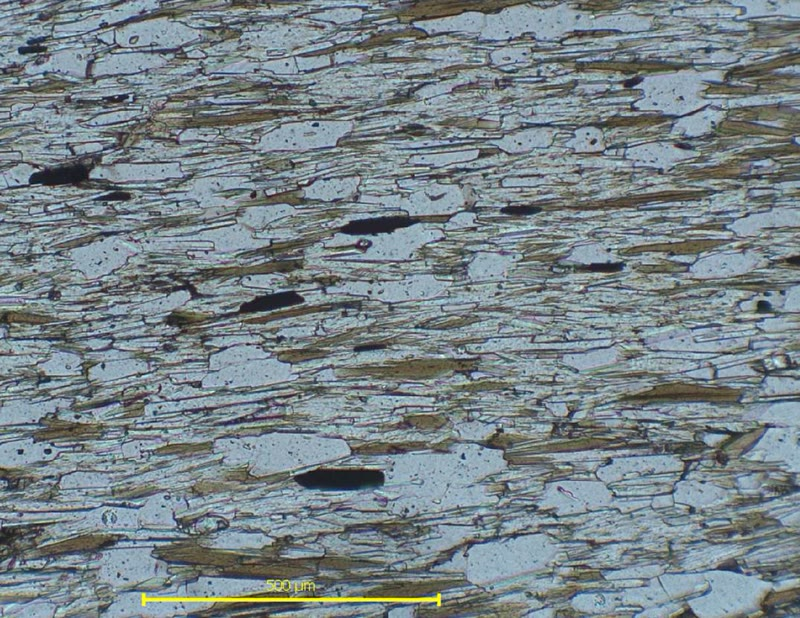
\includegraphics[height=4.3cm]{images/book2/g12-geoloshe-slaty-cleavage.jpg}\hspace{0.03\linewidth}%
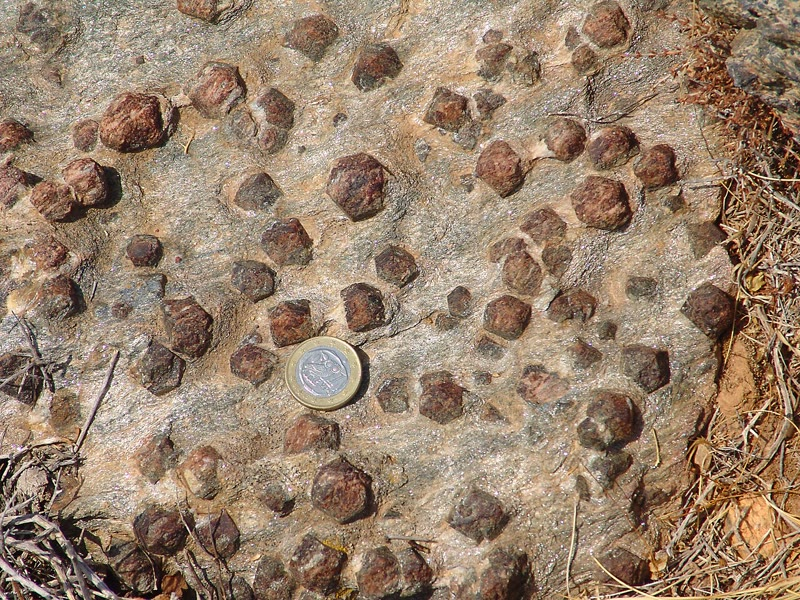
\includegraphics[height=4.3cm]{images/book2/g12-churchard-syros-garnet-schist.jpg}

\smallskip
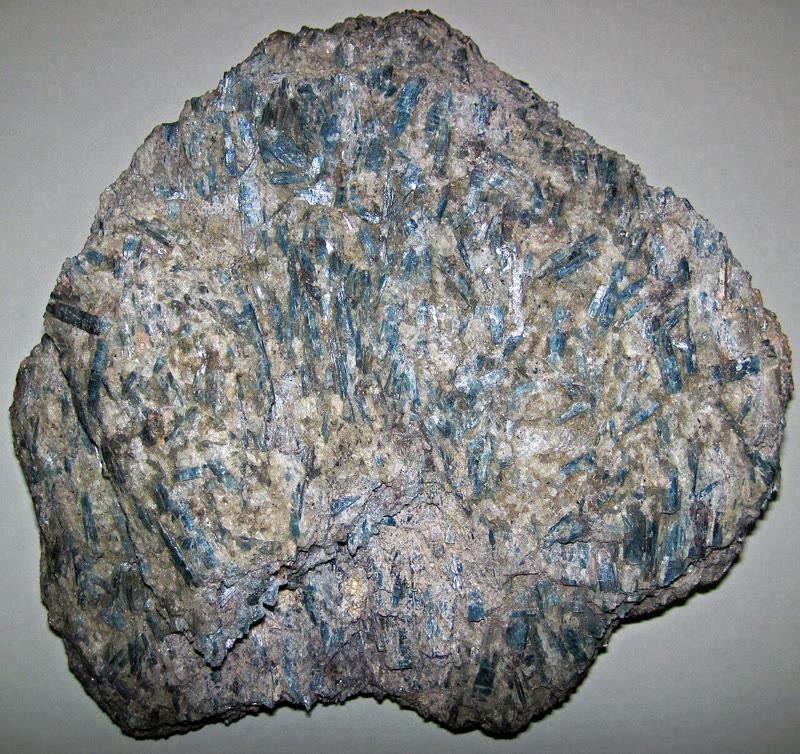
\includegraphics[height=4.3cm]{images/book2/g12-stjohn-kyanite-schist.jpg}\hspace{0.03\linewidth}%
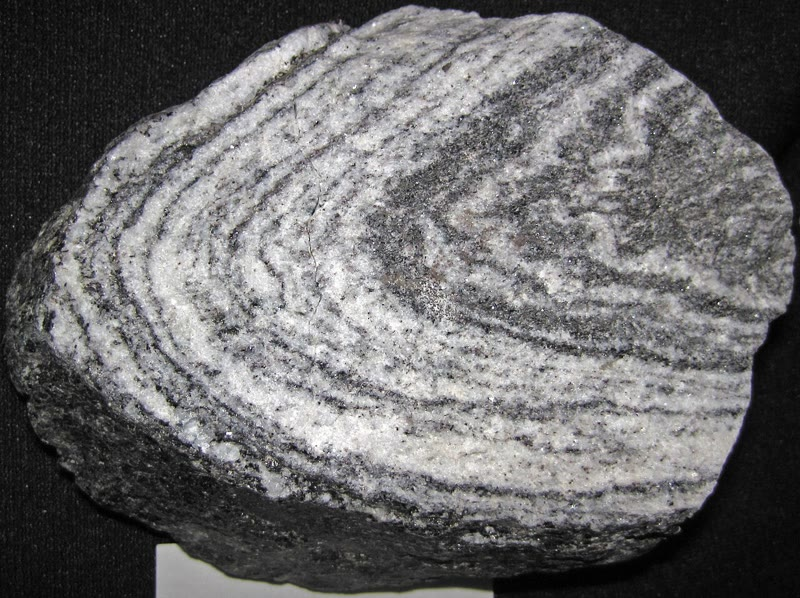
\includegraphics[height=4.3cm]{images/book2/g12-stjohn-gneiss.jpg}

{\small Em cima, à esquerda: uma ardósia ao microscópio (a barra amarela
mede \qty{500}{\micro\metre}): as suas escamas de mica estão todas
orientadas do mesmo modo. Em cima, à direita: um granada-mica xisto na ilha
de Siros; a moeda tem \qty{23}{mm} de diâmetro. Embaixo, à esquerda: um
xisto com lâminas azuis de cianita. Embaixo, à direita: um gnaisse com
faixas de quartzo (claras) e de mica biotita (escuras). Fotografias Geoloshe
(CC0), Graeme Churchard (CC~BY~2.0) e James St.~John (CC~BY~2.0).}
\end{omfigure}
% ledger: photo:g12-slaty-cleavage, photo:g12-syros-schist, photo:g12-kyanite-schist, photo:g12-gneiss

Ao longo de uma \omterm{def:g11:lithosphere-asthenosphere:geotherm}{geoterma} típica, a ardósia se forma entre cerca de 5 e
\qty{10}{km} de profundidade, o filito entre 10 e 15, o xisto entre 15 e
20, e o gnaisse entre 20 e \qty{25}{km}; mais fundo ainda, a rocha começa a
se fundir em alguns lugares. A \omterm{def:g12:metamorphic-rocks:foliation}{foliação} registra a direção da compressão:
ela se forma atravessada ao \omterm{def:g12:mountain-building:shortening}{encurtamento} que constrói as montanhas
(\cref{ch:g12:mountain-building}), e o acamamento original da lama ainda
pode ser visto cruzando-a em ângulo.
% ledger: earle:settings, earle:foliation

As rochas sem minerais achatados ou alongados não mostram \omterm{def:g12:metamorphic-rocks:foliation}{foliação} mesmo
quando são comprimidas. Um calcário vira um \textbf{mármore}, feito de
cristais maiores de calcita nos quais os fósseis foram apagados; um arenito
vira um \textbf{quartzito}, cujos grãos de quartzo cresceram uns dentro dos
outros; e uma lama aquecida sem ser comprimida vira uma rocha dura, de grão
fino, sem \omterm{def:g12:metamorphic-rocks:foliation}{foliação}, um \textbf{hornfels}.
% ledger: earle:foliation, earle:contact

\section{Metamorfismo de contato e metamorfismo regional}

\begin{definition}[Metamorfismo de contato; metamorfismo regional; auréola]\label{def:g12:metamorphic-rocks:contact-regional}
O \emph{metamorfismo de contato}\index{metamorfismo de contato} é o
\omterm{def:g12:metamorphic-rocks:metamorphism}{metamorfismo} das rochas aquecidas por um corpo de magma que se intrudiu
nelas; ele fica restrito a uma zona em volta da \omterm{def:g11:igneous-rocks:intrusion}{intrusão}, a sua
\emph{auréola}\index{aureola@auréola}, na qual o grau sobe em direção ao
contato. O \emph{metamorfismo regional}\index{metamorfismo regional} afeta
rochas enterradas a grande profundidade em grandes regiões, em geral onde as
placas convergem; as rochas são comprimidas além de aquecidas, e são quase
sempre foliadas.
\end{definition}
% ledger: earle:contact, earle:regional, tulane:metamorphism

\subsection{Em volta de um corpo de magma}

Um corpo de magma a cerca de \qty{1000}{\celsius} que sobe na crosta
superior fria aquece as rochas em volta dele. A sua temperatura pode chegar
de 300 a mais de \qty{800}{\celsius}, às baixas pressões das pequenas
profundidades. A \omterm{def:g12:metamorphic-rocks:contact-regional}{auréola} é estreita: alguns centímetros em volta de uma
lâmina fina de magma, até várias dezenas de metros em volta de um corpo
grande. As suas rochas são aquecidas sem ser comprimidas, por isso não são
foliadas: a lama vira hornfels, o calcário mármore, o arenito quartzito. Um
corpo de magma que se instala em profundidade em rochas que já estão
quentes quase não produz \omterm{def:g12:metamorphic-rocks:contact-regional}{auréola}.
% ledger: earle:contact, earle:settings (magma bodies around 1000 degC)

\begin{omfigure}
\begin{tikzpicture}[font=\scriptsize]
  \def\pluton{(3.0,0) .. controls (3.0,2.3) and (7.0,2.3) .. (7.0,0) -- cycle}
  \def\aureole{(2.45,0) .. controls (2.45,2.95) and (7.55,2.95) .. (7.55,0) -- cycle}
  \fill[lith sandstone] (0,0) rectangle (10,0.8);
  \fill[lith limestone] (0,0.8) rectangle (10,1.6);
  \fill[lith shale] (0,1.6) rectangle (10,3);
  \fill[omThm, opacity=0.30] \aureole;
  \draw[omThm, line width=0.6pt, dashed] (2.45,0) .. controls (2.45,2.95) and (7.55,2.95) .. (7.55,0);
  \fill[lith granite] \pluton;
  \draw[black!70, line width=0.6pt] (3.0,0) .. controls (3.0,2.3) and (7.0,2.3) .. (7.0,0);
  \draw[black!60] (0,0) rectangle (10,3);
  \node[fill=white, inner sep=1.5pt] at (5,0.45) {granito (antes magma)};
  \draw[black!70] (6.0,1.95) -- (10.6,2.4) node[right] {hornfels, a partir da lama};
  \draw[black!70] (7.0,1.2) -- (10.6,1.2) node[right] {mármore, a partir do calcário};
  \draw[black!70] (7.25,0.4) -- (10.6,0.4) node[right] {quartzito, a partir do arenito};
  \node[left] at (0,2.3) {folhelho};
  \node[left] at (0,1.2) {calcário};
  \node[left] at (0,0.4) {arenito};
  \draw[omThm] (4.2,2.05) -- (3.4,3.25) node[above, omThm] {auréola};
\end{tikzpicture}

{\small \omterm{def:g12:metamorphic-rocks:contact-regional}{Metamorfismo de contato}, em corte: um corpo de magma subiu em
rochas sedimentares acamadas e aqueceu uma \omterm{def:g12:metamorphic-rocks:contact-regional}{auréola} estreita (em vermelho)
em volta dele, cujas rochas se recristalizam sem ser comprimidas.
Esquemático: as \omterm{def:g12:metamorphic-rocks:contact-regional}{auréolas} reais têm de centímetros a dezenas de metros de
largura.}
\end{omfigure}
% ledger: earle:contact

\subsection{Sob um cinturão de montanhas}

O \omterm{def:g12:metamorphic-rocks:contact-regional}{metamorfismo regional} exige um soterramento a 10 ou \qty{20}{km}, por
isso ele afeta milhares de quilômetros quadrados de uma vez. O lugar mais
provável é a \omterm{def:g12:continental-crust:root}{raiz} de um cinturão de montanhas, onde a colisão espessa a
crosta e empurra as suas rochas para baixo
(\cref{ch:g12:mountain-building}). Num antigo cinturão cujas zonas foram
mapeadas, as rochas da zona da silimanita foram aquecidas acima de
\qty{700}{\celsius} e enterradas de 20 a \qty{25}{km} de profundidade,
enquanto as da zona externa da clorita provavelmente nunca foram enterradas
a mais de cerca de \qty{5}{km}. As montanhas de cima foram depois
desgastadas ao longo de dezenas de milhões de anos; à medida que a carga era
removida, a crosta espessa voltou a subir, e as zonas antes profundas estão
hoje na superfície (\cref{ch:g12:destruction-of-mountains}).
% ledger: earle:regional

\subsection{Três geotermas}

Os \omterm{def:g12:metamorphic-rocks:polymorph}{polimorfos} mostram num relance que a mesma profundidade não significa a
mesma rocha em toda parte: isso depende da \omterm{def:g11:lithosphere-asthenosphere:geotherm}{geoterma}. A figura dos
\omterm{def:g12:metamorphic-rocks:polymorph}{polimorfos} traz três delas.
% ledger: earle:settings

\begin{itemize}
  \item Uma \omterm{def:g11:lithosphere-asthenosphere:geotherm}{geoterma} \textbf{típica}, cerca de \qty{30}{\celsius} por
        quilômetro: a temperatura chega a cerca de \qty{300}{\celsius} a
        \qty{10}{km}. Ela passa abaixo do ponto triplo, então a cianita dá
        lugar diretamente à silimanita, a cerca de \qty{574}{\celsius} e
        \qty{18.8}{km}.
  \item Uma \omterm{def:g11:lithosphere-asthenosphere:geotherm}{geoterma} de \textbf{região vulcânica}, de 40 a
        \qty{50}{\celsius} por quilômetro, tornada mais íngreme pelo calor
        do magma que sobe: as rochas atingem altas temperaturas a pequenas
        profundidades. A \qty{50}{\celsius} por quilômetro, a andaluzita
        aparece a cerca de \qty{6.6}{km} e dá lugar à silimanita a cerca de
        \qty{10.9}{km}, \qty{553}{\celsius}.
  \item A \omterm{def:g11:lithosphere-asthenosphere:geotherm}{geoterma} de uma \textbf{\omterm{def:g11:subduction-zones:subduction}{zona de subducção}}, abaixo de
        \qty{10}{\celsius} por quilômetro: a \omterm{def:g11:ocean-ridges:oceanic-lithosphere}{crosta oceânica} levada para
        baixo continua várias centenas de graus mais fria que o manto em
        volta. A \qty{36}{km}, ela está só a cerca de \qty{370}{\celsius},
        bem dentro do campo da cianita. É o caminho frio, de alta pressão,
        no qual o basalto vira \omterm{def:g11:subduction-zones:eclogite}{xisto azul}, depois \omterm{def:g11:subduction-zones:eclogite}{eclogito}, a cerca de
        \qty{35}{km}.
\end{itemize}
% values: cross_30_0 573.6 degC 18.79 km; cross_50_0 340.1 degC 6.60 km; cross_50_1 553.0 degC 10.86 km; sub10_T_at_1gpa 370.2 (al2sio5.py)
% ledger: earle:settings

Assim, cada rocha metamórfica traz um registro da \omterm{def:g11:lithosphere-asthenosphere:geotherm}{geoterma} sob a qual se
formou, e do contexto de placas por trás dela: a andaluzita e o hornfels
apontam para calor a pequenas profundidades, em volta de corpos de magma; os
xistos e os gnaisses com cianita e silimanita, para as \omterm{def:g12:continental-crust:root}{raízes} profundas dos
cinturões de montanhas; os \omterm{def:g11:subduction-zones:eclogite}{xistos azuis} e os \omterm{def:g11:subduction-zones:eclogite}{eclogitos}, para as \omterm{def:g11:subduction-zones:subduction}{zonas de
subducção}. A maioria dessas rochas só pôde ser vista porque voltou à
superfície sem se transformar de volta. À medida que sobem e esfriam, as
suas reações ficam mais lentas, e a água de que as reações inversas
precisariam escapou na descida.
% ledger: earle:settings, earle:contact, tulane:metamorphism (retrograde metamorphism uncommon)

\section{Exercícios}

\begin{exercise}[$\star$]\label{exo:g12:metamorphic-rocks:1}
Dê a palavra: (a) minerais de mesma composição mas de estruturas
cristalinas diferentes; (b) a linha num mapa onde um \omterm{def:g12:metamorphic-rocks:index-mineral}{mineral índice} aparece
pela primeira vez; (c) a zona de rochas aquecidas em volta de um corpo de
magma; (d) os planos paralelos formados por minerais achatados alinhados;
(e) a pressão devida ao peso das rochas de cima.
\end{exercise}

\begin{exercise}[$\star$]\label{exo:g12:metamorphic-rocks:2}
Dê o nome da rocha metamórfica em que cada \omterm{def:g10:soil-formation:weathering-profile}{rocha-mãe} se transforma: (1) um
calcário; (2) um arenito; (3) uma lama, em grau baixo sob compressão; (4)
uma lama, em grau alto; (5) uma lama, aquecida por um corpo de magma sem
ser comprimida.
\end{exercise}

\begin{exercise}[$\star$]\label{exo:g12:metamorphic-rocks:3}
Com $\rho = \qty{2830}{kg/m^3}$ e $g = \qty{9.81}{m/s^2}$, calcule a
\omterm{def:g12:metamorphic-rocks:lithostatic}{pressão litostática}, em \unit{GPa}, a \qty{10}{km} e a \qty{20}{km}.
\end{exercise}

\begin{exercise}[$\star$]\label{exo:g12:metamorphic-rocks:4}
No diagrama dos \omterm{def:g12:metamorphic-rocks:polymorph}{polimorfos} de \ce{Al2SiO5}, que mineral é estável (1) a
\qty{400}{\celsius} e \qty{0.6}{GPa}; (2) a \qty{500}{\celsius} e
\qty{0.2}{GPa}; (3) a \qty{750}{\celsius} e \qty{0.3}{GPa}?
\end{exercise}

\begin{exercise}[$\star$]\label{exo:g12:metamorphic-rocks:5}
(1) Ponha em ordem crescente de grau: xisto, ardósia, gnaisse, filito. (2)
Em qual delas as micas podem ser vistas a olho nu? (3) Qual mostra faixas
claras e escuras?
\end{exercise}

\begin{exercise}[$\star\star$]\label{exo:g12:metamorphic-rocks:6}
(1) Calcule a \omterm{def:g12:metamorphic-rocks:lithostatic}{pressão litostática} na base de uma crosta de \qty{35}{km} de
espessura ($\rho = \qty{2830}{kg/m^3}$) e expresse-a em atmosferas
($\qty{1}{atm} = \qty{101325}{Pa}$). (2) Calcule a pressão no fundo de um
oceano de \qty{4}{km} de profundidade, com uma água do mar de densidade
\qty{1025}{kg/m^3}. (3) Quantas vezes a primeira é maior?
\end{exercise}

\begin{exercise}[$\star\star$]\label{exo:g12:metamorphic-rocks:7}
O ponto triplo de \ce{Al2SiO5} fica a \qty{504}{\celsius} e
\qty{0.375}{GPa}. (1) A que profundidade essa pressão é atingida ($\rho =
\qty{2830}{kg/m^3}$)? (2) Que \omterm{def:g11:lithosphere-asthenosphere:geotherm}{gradiente geotérmico}, partindo de
\qty{10}{\celsius} na superfície, passa exatamente por ele? (3) Uma rocha que
contém os três \omterm{def:g12:metamorphic-rocks:polymorph}{polimorfos} tem chance de ser comum?
\end{exercise}

\begin{exercise}[$\star\star$]\label{exo:g12:metamorphic-rocks:8}
Na fotografia do granada xisto de Siros, as maiores granadas têm cerca de
um terço do diâmetro da moeda, que mede \qty{23}{mm}. (1) Estime o seu
diâmetro. (2) Se o diâmetro de uma granada cresce cerca de \qty{1}{mm} em
um milhão de anos, quanto tempo elas levaram para crescer? (3) O que isso
diz sobre o tempo que uma rocha passa em profundidade?
\end{exercise}

\begin{exercise}[$\star\star$]\label{exo:g12:metamorphic-rocks:9}
Percorrendo \qty{24}{km} para oeste através de um antigo cinturão de
montanhas, um geólogo registra rochas formadas a partir de lama. No início,
elas contêm só clorita e biotita; a primeira granada aparece depois de
\qty{6}{km}, a primeira estaurolita depois de \qty{11}{km}, a primeira
cianita depois de \qty{15}{km}, a primeira silimanita depois de
\qty{20}{km}. (1) Quantas \omterm{def:g12:metamorphic-rocks:index-mineral}{isógradas} foram cruzadas? Cite-as em ordem.
(2) Em que direção o grau sobe? (3) Onde as rochas foram enterradas mais
fundo, e aproximadamente quão quentes elas ficaram ali?
\end{exercise}

\begin{exercise}[$\star\star$]\label{exo:g12:metamorphic-rocks:10}
Um corpo de magma sobe em camadas de lama, de calcário e de arenito perto da
superfície. (1) Dê o nome da rocha em que cada camada se transforma junto a
ele. (2) Por que essas rochas não são foliadas? (3) Um segundo corpo de
magma se instala a \qty{20}{km} de profundidade, em rochas que já estão
perto de \qty{500}{\celsius}. Por que ele quase não produz \omterm{def:g12:metamorphic-rocks:contact-regional}{auréola}?
\end{exercise}

\begin{exercise}[$\star\star$]\label{exo:g12:metamorphic-rocks:11}
Uma camada de lama é comprimida a partir do leste e do oeste durante uma
colisão, e faz crescer micas à medida que é aquecida. (1) Como as micas se
dispõem: com as suas faces planas voltadas para leste--oeste ou para
norte--sul? (2) A \omterm{def:g12:metamorphic-rocks:foliation}{foliação} que se forma é horizontal ou vertical? (3) Um
mármore e um quartzito comprimidos da mesma maneira não mostram \omterm{def:g12:metamorphic-rocks:foliation}{foliação}.
Por quê?
\end{exercise}

\begin{exercise}[$\star\star\star$]\label{exo:g12:metamorphic-rocks:12}
Entre 500 e \qty{700}{\celsius}, o limite cianita--silimanita é próximo da
reta $P = 0.577 + 0.00209\,(T - 600)$, com $P$ em
\unit{GPa} e $T$ em \unit{\celsius}. Uma \omterm{def:g11:lithosphere-asthenosphere:geotherm}{geoterma} típica é $T = 10 + 30z$
($z$ em \unit{km}), e $P = 0.0278\,z$. (1) Escreva a \omterm{def:g11:lithosphere-asthenosphere:geotherm}{geoterma} como $P$ em
função de $T$. (2) Encontre onde ela cruza o limite: temperatura, pressão,
profundidade. (3) Ao longo dessa \omterm{def:g11:lithosphere-asthenosphere:geotherm}{geoterma}, que \omterm{def:g12:metamorphic-rocks:polymorph}{polimorfo} é estável logo
acima dessa profundidade, e qual logo abaixo?
\end{exercise}

\begin{exercise}[$\star\star\star$]\label{exo:g12:metamorphic-rocks:13}
(1) Ao longo de uma \omterm{def:g11:lithosphere-asthenosphere:geotherm}{geoterma} de \omterm{def:g11:subduction-zones:subduction}{subducção} de \qty{10}{\celsius} por
quilômetro, partindo de \qty{10}{\celsius}, qual é a temperatura a
\qty{35}{km}, onde o \omterm{def:g11:subduction-zones:eclogite}{eclogito} se forma? (2) Qual é ela ao longo de uma
\omterm{def:g11:lithosphere-asthenosphere:geotherm}{geoterma} típica de \qty{30}{\celsius} por quilômetro? (3) Situe os dois
pontos no diagrama dos \omterm{def:g12:metamorphic-rocks:polymorph}{polimorfos}: que \omterm{def:g12:metamorphic-rocks:polymorph}{polimorfo} é estável no primeiro?
(4) Por que os \omterm{def:g11:subduction-zones:eclogite}{xistos azuis} e os \omterm{def:g11:subduction-zones:eclogite}{eclogitos} se formam nas \omterm{def:g11:subduction-zones:subduction}{zonas de subducção}
e quase em nenhum outro lugar?
\end{exercise}

\begin{exercise}[$\star\star\star$]\label{exo:g12:metamorphic-rocks:14}
As densidades da cianita, da silimanita e da andaluzita são \num{3.61},
\num{3.24} e \qty{3.15}{g/cm^3}. (1) Calcule o volume de \qty{1}{kg} de
cada uma, em \unit{cm^3}. (2) Em que porcentagem a cianita é menor que a
andaluzita de mesma massa? (3) Explique, com a ideia de que uma alta pressão
favorece o arranjo que ocupa menos espaço, por que a cianita ocupa o campo
de alta pressão do diagrama.
\end{exercise}

\begin{exercise}[$\star\star\star$]\label{exo:g12:metamorphic-rocks:15}
Num antigo cinturão de montanhas, as rochas da zona da silimanita foram
aquecidas acima de \qty{700}{\celsius} e enterradas de 20 a \qty{25}{km} de
profundidade. (1) Calcule a pressão a 20 e a \qty{25}{km}. (2) Usando a
reta do exercício~12, encontre a temperatura mais baixa em que a silimanita é
estável a cada uma dessas pressões. \qty{700}{\celsius} é coerente com a
silimanita? (3) Que \omterm{def:g11:lithosphere-asthenosphere:geotherm}{gradientes geotérmicos}, a partir de \qty{10}{\celsius}
na superfície, \qty{700}{\celsius} a 20 e a \qty{25}{km} implicam? (4) As
rochas afloraram na superfície cerca de 40 milhões de anos depois. A que
taxa média a rocha acima delas foi removida, em \unit{mm} por ano?
\end{exercise}

\begin{problem}[{Problema de fim de semana --- a história de um xisto com cianita}]
\label{pb:g12:metamorphic-rocks:1}
% ledger: hm93:table11, cm95:crust, earle:controls, earle:settings, earle:regional, tulane:roots, tulane:metamorphism, iugs:barrow; Book 3: webmineral:polymorphs; Book 1: ussa76:sea-level
% values: pb_z_km 25.214, pb_grad 23.4, pb_kysil_P_at_600_gpa 0.577 (al2sio5.py); t_on_kysil(7.0) = 658.9
Um xisto coletado no núcleo de um antigo cinturão de montanhas contém
muscovita, biotita, quartzo, granadas de até \qty{8}{mm} de diâmetro e
lâminas azuis de cianita; ele não contém nem silimanita nem andaluzita.
Análises de laboratório da sua granada e da sua biotita dão as condições em
que ele se cristalizou: cerca de \qty{600}{\celsius} e \qty{0.70}{GPa}. Tome
$\rho =
\qty{2830}{kg/m^3}$, $g = \qty{9.81}{m/s^2}$, \qty{10}{\celsius} na
superfície, e a reta cianita--silimanita do exercício~12, $P = 0.577 +
0.00209\,(T - 600)$.

\medskip
\noindent\textbf{Parte I --- Os minerais.}
\begin{enumerate}
  \item Por que a rocha se chama xisto? Quais dos seus minerais formam a
        \omterm{def:g12:metamorphic-rocks:foliation}{xistosidade}?
  \item A cianita, a andaluzita e a silimanita compartilham uma fórmula.
        Escreva-a, e dê a palavra para esses minerais.
  \item As densidades da cianita e da andaluzita são \num{3.61} e
        \qty{3.15}{g/cm^3}. Em que porcentagem o volume de um quilograma de
        cianita é menor? Qual delas a pressão favorece?
  \item Na sequência dos \omterm{def:g12:metamorphic-rocks:index-mineral}{minerais índice} das rochas formadas a partir de
        lama, a que zona a rocha pertence? Que \omterm{def:g12:metamorphic-rocks:index-mineral}{isógradas} ela cruzou na
        descida?
  \item Se o diâmetro das granadas cresceu cerca de \qty{1}{mm} em um milhão
        de anos, quanto tempo as maiores levaram para crescer?
\end{enumerate}

\medskip
\noindent\textbf{Parte II --- Pressão e temperatura.}
\begin{enumerate}[resume]
  \item A \qty{600}{\celsius}, acima de que pressão a cianita é estável, em
        vez da silimanita?
  \item Verifique que o ponto (\qty{600}{\celsius}, \qty{0.70}{GPa}) fica no
        campo da cianita.
  \item A falta de silimanita dá uma pressão mínima a \qty{600}{\celsius}.
        Qual é?
  \item Se a rocha tivesse sido mais aquecida a \qty{0.70}{GPa}, a que
        temperatura a sua cianita teria se transformado em silimanita?
  \item Expresse \qty{0.70}{GPa} em quilobars ($\qty{1}{kbar} =
        \qty{e8}{Pa}$) e em atmosferas ($\qty{1}{atm} = \qty{101325}{Pa}$).
\end{enumerate}

\medskip
\noindent\textbf{Parte III --- A profundidade de soterramento.}
\begin{enumerate}[resume]
  \item Em quantos megapascals a \omterm{def:g12:metamorphic-rocks:lithostatic}{pressão litostática} sobe por quilômetro?
  \item A que profundidade estava o xisto quando se cristalizou?
  \item Qual é a menor profundidade permitida pela falta de silimanita
        (questão 8)?
  \item Refaça a questão 12 com uma densidade de \qty{2700}{kg/m^3} para as
        rochas de cima. Em que porcentagem a profundidade muda?
  \item Uma \omterm{def:g12:continental-crust:continental-crust}{crosta continental} tem normalmente de 35 a \qty{40}{km} de
        espessura, e de 50 a \qty{70}{km} sob os cinturões de montanhas. O
        xisto se cristalizou na crosta ou no manto?
\end{enumerate}

\medskip
\noindent\textbf{Parte IV --- A geoterma, e o caminho de volta.}
\begin{enumerate}[resume]
  \item Que \omterm{def:g11:lithosphere-asthenosphere:geotherm}{gradiente geotérmico} médio \qty{600}{\celsius} a essa
        profundidade implicam?
  \item Compare-o com os gradientes de uma \omterm{def:g11:subduction-zones:subduction}{zona de subducção}, de uma crosta
        típica e de uma região vulcânica. Que tipo de \omterm{def:g12:metamorphic-rocks:metamorphism}{metamorfismo} formou a
        rocha?
  \item Ao longo de uma \omterm{def:g11:lithosphere-asthenosphere:geotherm}{geoterma} típica de \qty{30}{\celsius} por
        quilômetro, qual seria a temperatura à profundidade da questão 12?
        Que \omterm{def:g12:metamorphic-rocks:polymorph}{polimorfo} seria então estável a \qty{0.70}{GPa}?
  \item Para trazer o xisto à superfície, toda a rocha acima dele teve de
        ser removida. A uma taxa média de \qty{0.5}{mm} por ano, quanto tempo
        isso levou?
  \item Por que a cianita não voltou a se transformar em andaluzita na
        subida?
  \item Resuma: a que profundidade este xisto com cianita se cristalizou?
\end{enumerate}
\end{problem}
